\section{Netzwerksniffer-Projekt im Karosseriebau der Porsche AG}

\subsection{Problemstellung und Ziel}
Im Produktionsumfeld der Porsche AG soll das Asset Inventory vorangetrieben werden. Um eine effektive Schutzstrategie zu gestalten, ist es notwendig, sämtliche OT-Geräte-Attribute systematisch zu erfassen, da nur bekannte Objekte angemessen geschützt werden können. Dabei ist es entscheidend, die Verfügbarkeit jederzeit sicherzustellen, da diese für den Produktionsbetrieb unerlässlich ist. Ein strukturiertes Asset Management bildet somit das Fundament, um die Sicherheit in der Produktion vor Cyberangriffen zu gewährleisten. Um möglichst viele OT-Geräte-Attribute erfassen zu können, wird ein passiver Netzwerksniffer eingesetzt. Die Entscheidung für eine passive Methode basiert auf der Tatsache, dass im Produktionsbereich das Schutzziel der Verfügbarkeit höchste Priorität hat. Der Einsatz aktiver Scanner wäre riskant, da diese potenziell störend auf die empfindlichen und oft zeitkritischen Systeme wirken könnten. Aktive Scanner senden Anfragen an Geräte im Netzwerk, um Informationen über deren Zustand oder Konfiguration zu sammeln. Diese zusätzlichen Anfragen können die Netzwerklast erhöhen und zu Verzögerungen oder sogar Unterbrechungen in der Kommunikation zwischen den Steuerungssystemen führen. Im Gegensatz dazu überwachen passive Scanner den Netzwerkverkehr, indem sie die Kommunikation beobachten, ohne aktiv einzugreifen. Dies hat den Vorteil, dass das Netzwerk nicht zusätzlich belastet wird und die regulären Betriebsabläufe ungestört bleiben. Allerdings ist die Datenerfassung durch passive Sniffer zeitaufwändiger, da sie darauf angewiesen sind, dass die OT-Geräte selbstständig Datenverkehr generieren, um die benötigten Informationen zu sammeln (vgl. \cite{aktivScan}). Zusammenfassend lässt sich feststellen, dass die Kombination passiver und aktiver Methoden eine effektive Strategie zur Verbesserung des Asset Inventory in der Produktion darstellt. Aktive Scans können insbesondere während Betriebsruhezeiten eingesetzt werden, wenn die Produktion ohnehin stillsteht, um OT-Geräte-Attribute zuverlässig zu erfassen. Da jedoch aktive Scans im laufenden Betrieb potenzielle Störungen verursachen können, ist der Einsatz passiver Scans in diesen Phasen vorzuziehen, um die Betriebskontinuität zu gewährleisten. In einem Feldversuch wird nun in einer repräsentativen Automatisierungstestzelle bei der Porsche AG ein Netzwerksniffer eingesetzt, um eine möglichst umfassende Erfassung der erforderlichen OT-Geräte-Attribute durch passive Netzwerksniffer zu erreichen. Die Testzelle, die den tatsächlichen Produktionsbedingungen sehr ähnlich ist und PROFINET als Kommunikationsstandard verwendet, bildet eine geeignete Umgebung für diesen Zweck. Bei der Auswahl der passiven Netzwerksniffer wurde berücksichtigt, dass PROFINET der relevante Kommunikationsstandard ist. Die Leistungsfähigkeit des Netzwerksniffers wird durch die Analyse und Bewertung der erfassten OT-Geräte-Attribute beurteilt. Diese Ergebnisse sollen auf die realen Produktionszellen übertragbar sein. Auf Basis der erhaltenen Resultate wird entschieden, ob der eingesetzte Netzwerksniffer geeignet ist, das Asset Inventory in der Produktionsumgebung zu optimieren und voranzutreiben. Es findet ein Vergleich der Erkennungsgrade zwischen der VW-Eigenentwicklung Distributed Plant Monitor (DPM) und dem Netzwerksniffer PROFINET INspektor der Firma Indu-Sol statt.

\subsection{OT-Asset-Inventory}

  „Ein OT-Asset [...] ist jede Art von Informationen oder Daten, Software oder Hardware, die ein Unternehmen im Rahmen seiner Geschäftstätigkeit nutzt.'' (\cite{IBM})

\ac{itam} bezieht sich auf die vollständige Nachverfolgung und Verwaltung von OT-Assets. Es stellt sicher, dass jedes OT-Asset effizient genutzt, ordnungsgemäß gewartet, regelmäßig aktualisiert und am Ende seiner Lebensdauer angemessen entsorgt wird (vgl. \cite{IBM}). Das OT-Asset-Management ist niemals ein zeitlich terminiertes Projekt, sondern ein Prozess, der regelmäßig durchgeführt werden muss, um einen aktuellen Stand zu wahren. In diesem Prozess unterteilt man die folgenden Schritte: Zu Beginn wird ein detailliertes Inventar aller OT-Assets erstellt. Im Inventar werden die gekauften OT-Assets nach Kriterien aufgelistet, welche variabel festgelegt werden können. Besonders im Bereich der OT sind sinnvolle Kriterien beispielsweise der Name des OT-Assets, der Gerätetyp, die IP-Adresse, der Standort, die Seriennummer oder auch Hersteller und Wartungsstatus des Geräts. Grundsätzlich können diese je nach Anwendung variabel gesetzt werden. Im Bereich der industriellen Cybersicherheit ist ein detailliertes OT-Asset-Inventar von entscheidender Bedeutung. Eine adäquate Sicherung von OT-Geräten und zugehöriger Software ist nur möglich, wenn diese umfassend erfasst und dokumentiert sind (\cite{atlassian}). Eine strukturierte Liste aller Geräte im Automationsnetz ermöglicht die Entwicklung effektiver Schutzkonzepte. Ein umfassendes Inventar sollte zusätzliche Informationen wie Softwarestand, Version und Betriebssystem enthalten, um grundlegende Schwachstellen schnell diagnostizieren zu können. Ein weiterer Vorteil liegt in den Kosteneinsparungen, die durch ein sorgfältig geführtes Inventar erzielt werden. Dies trägt zur Vermeidung unnötiger Anschaffungen bei und optimiert die Nutzung vorhandener Ressourcen. Zudem ermöglicht die gewonnene Transparenz eine bessere Planung und Durchführung von Wartungsarbeiten (vgl. \cite{sichereIndustrie}). Im Folgenden ist dies von besonderer Bedeutung für diese Projektarbeit, da im weiteren Verlauf eine Technologie präsentiert wird, welche die Verbesserung dieses Prozesses ermöglicht. Daraufhin folgt die Anlagenwartung, welche "[...] die Reparatur, die Aktualisierung und den Austausch von Assets umfasst" (\cite{IBM}).
\clearpage

\subsection{PROFINET-Inspektor (Indu-Sol) und DPM}

PROFINET ist ein Industrial-Ethernet-Standard, der speziell für Anwendungen in der industriellen Automatisierung, einschließlich der Fertigungs- und Prozessautomatisierung, entwickelt wurde. Er ermöglicht die deterministische Datenkommunikation\footnote{bevor auf das Netzwerk zugegriffen werden kann, muss eine Rechtevergabe erfolgen, bei der nur ein Host das Senderecht und die Nutzung eines Kanals zugesichert bekommt} und zeichnet sich durch seine Modularität und Unterstützung verschiedener Übertragungsmedien aus, wobei er auf TCP/IP basiert. PROFINET definiert vier aufeinander aufbauende Konformitätsklassen (Conformance Classes, CC). Diese Klassen sind jeweils spezifisch auf den entsprechenden Einsatzzweck abgestimmt (vgl. \cite{IPInsider}):

\begin{itemize}
\item \textbf{CC-A} enthält Grundfunktionen.
\item \textbf{CC-B} erweitert CC-A um Netzwerkdiagnose und Topologie-Informationen.
\item \textbf{CC-C} umfasst eine Erweiterung zur Implementierung von IRT-Kommunikation\footnote{(Isochronous Real-Time Communication) synchronisiertes Übertragungsverfahren, das für den zyklischen Austausch von Daten zwischen PROFINET-Geräten verwendet wird}, die die Grundlage für taktsynchrone Anwendungen bildet.
\item \textbf{CC-D} erweitert die Klasse C, indem es dieselben Dienste unter Verwendung der von IEEE (Institute of Electrical and Electronics Engineers) definierten Mechanismen des TSN (Time-Sensitive Networking) bereitstellt.
\end{itemize} PROFINET nutzt ein einfaches 4-schichtiges TCP/IP-Modell. Der PROFINET INspektor® der Marke Indu-Sol überwacht und speichert teilnehmerbezogene Ereignisse in PROFINET-Netzwerken basierend auf vordefinierten Triggerfunktionen. Es handelt sich dabei um einen Netzwerksniffer, welcher den Datenverkehr in einer Netwzerkverbindung mitlesen kann und dessen Analyse ermöglicht.  Auf diese Art und Weise kann er spezifische Informationen wie IP-Adressen, Portnummern sowie den Inhalt übertragener Nachrichten erfassen. Diese Daten ermöglichen es, den Netzwerkverkehr im Detail zu verstehen, diesen zu überwachen und potenzielle Probleme frühzeitig zu erkennen (vgl. \cite{luber}). Die OT-Geräte-Attribute werden dabei über die XML-basierten GSDML-Dateien erfasst.  \ac{gsdml} ist eine Sprache zur Beschreibung von PROFINET IO-Feldgeräten. Ein Netzwerksniffer erfasst den Datenverkehr und identifiziert OT-Geräte. Sobald ein Gerät identifiziert wurde, kann der Sniffer die GSDML-Datei laden. Das ist möglich, da die GSDML-Dateien standardisiert sind und Attribute wie die Geräte-Identifikationsnumer enthalten. Schließlich kann der Sniffer diese GSDML-Dateien analysieren und die Ergebnisse in Form von OT-Geräte-Attributen (IP-Adresse, MAC-Adresse etc.) ausgeben (vgl. \cite{SIEMENS}). \clearpage \noindent Dabei liefert das Gerät wichtige Informationen zu Qualitätsmerkmalen wie Netzwerkbelastung, Datenfluss, Aktualisierungsintervallen, Lücken in der Übertragung und Schwankungen in den Telegrammzeiten, die den aktuellen Zustand der Kommunikationsqualität im Netzwerk darstellen. Ein solcher Qualitätscheck des PROFINET-Netzwerks, der diese Parameter berücksichtigt, ist nicht nur als Abnahme- und Prüfungsinstrument bei neuen Installationen von Bedeutung, sondern liefert auch wertvolle Daten für die Wartung, Instandhaltung und den (Remote-)Service. Der integrierte Webserver bietet die Möglichkeit, die Netzwerkdaten übersichtlich darzustellen (vgl. \cite{InduSol}).
\begin{figure}[H]
    \centering
    \includegraphics[width=0.29\textwidth]{images/PROFINET-INspektor.jpg}
    \caption{PROFINET-INspektor® NT im Schaltschrank, Porsche AG (eigene Aufnahme)}
    \label{fig:PROFINET-INspektor® NT}
\end{figure} 
Der \ac{dpm} ist eine Eigenentwicklung des VW-Konzerns. Dabei handelt es sich um ein System zur aktiven Diagnose von Anlagennetzen mit Ethernetgeräten wie PROFINET. Es sammelt und analysiert Assetinformationen, Konfigurationen und Metriken, um Berichte zu erstellen. 
Zu den Hauptfunktionen zählen das Asset-Management, die Überprüfung von Gerätekonfigurationen, die Überwachung der Netzwerkgüte und die Kontrolle der Netzwerktopologie. DPM besteht aus verschiedenen Komponenten: Clients (Agents) in den Subnetzen, die Informationen sammeln, einem Server, der diese Informationen verarbeitet und speichert, und einer zentralen Datenbank. Für die Anwender steht ein Web-Interface zur Verwaltung und Ansicht der gesammelten Daten zur Verfügung. Die wesentliche Unterscheidung beider Geräte liegt in der Eigenschaft, dass das Gerät der Firma Indu-Sol passiv agiert, während die VW-Eigenentwicklung aktive und passive Elemente kombiniert. 

\subsection{Analyse und Bewertung der Ergebnisse}

DPM und Indu-Sol haben die OT-Geräte-Attribute MAC-Adresse, IP-Adresse, Name, Gerätetyp, Bestellnummer, Hardware-Version, Firmware-Version, Subnetz, Gateway und Seriennummer erfasst. Die Werte wurden über die Weboberfläche der jeweiligen Sniffer erfasst und in einer Excel-Tabelle verglichen. Bei der Auswertung stellt man fest, dass beide Systeme grundsätzlich hohe Erkennungsgrade aufweisen.  Bei der Erfassung von Insgesamt 97 OT-Geräten erfasst DPM in der Summe jedoch 13,92\%\ mehr Daten als der PROFINET Inspektor von Indu-Sol. 
Die Kompetenzen der beiden Systeme sind dennoch unterschiedlich verteilt. Hervorzuheben ist auch, dass der PROFINET Inspektor keine Seriennummern erfasst hat. Bei Außerachtlassung dieses Attributs, würde diese Diskrepanz bei 0,4\%\ liegen, wodurch beide Systeme über einen vergleichbaren Erkennungsgrad verfügen würden.  


\noindent Das folgende Diagramm zeigt visuell den Unterschied hinsichtlich Erkennungsgrad zwischen dem Indu-Sol Profinet Inspektor und dem DPM-System in den jeweiligen Attributen in der Produktion der Porsche AG auf:


\bigskip
\begin{figure}[h]
    \centering
    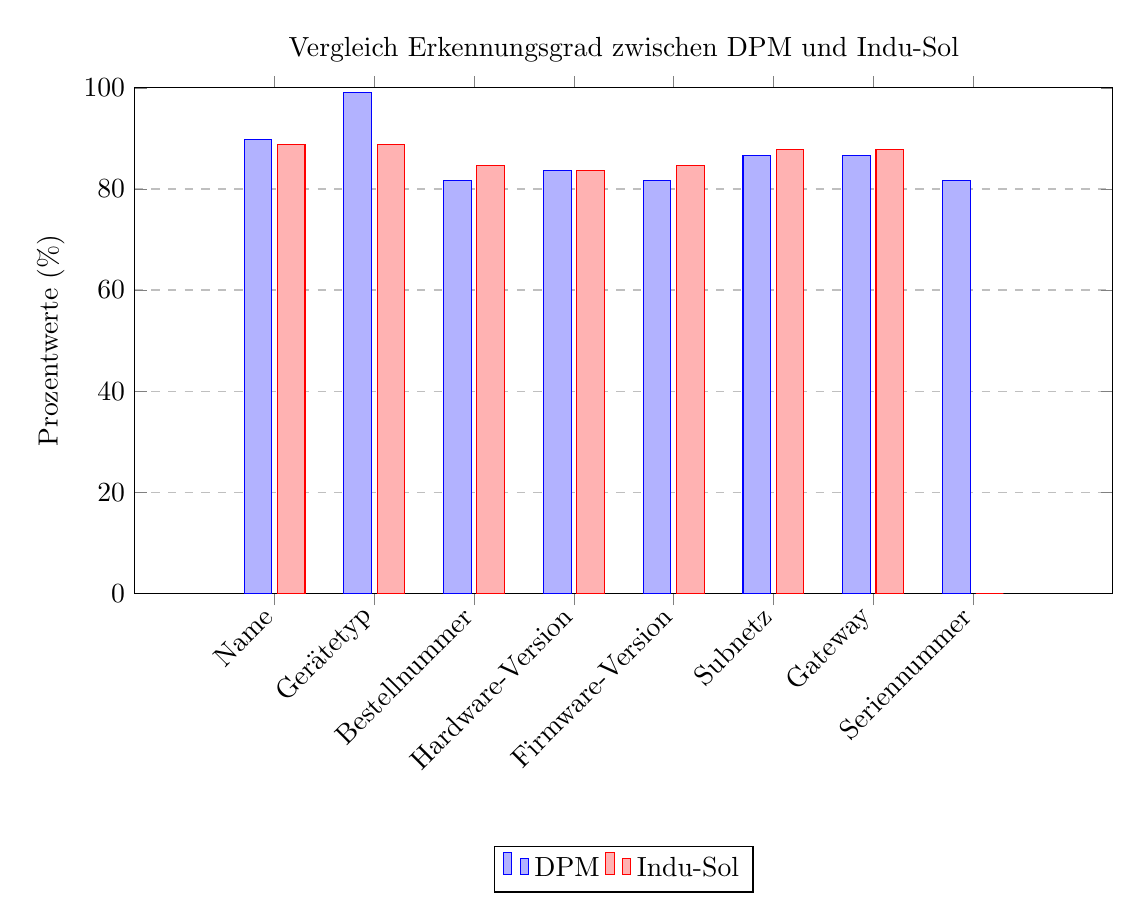
\begin{tikzpicture}
        \begin{axis}[
            title={Vergleich Erkennungsgrad zwischen DPM und Indu-Sol},
            ybar,
            symbolic x coords={Name, Gerätetyp, Bestellnummer, Hardware-Version, Firmware-Version, Subnetz, Gateway, Seriennummer},
            xtick=data,
            ymin=0,
            ymax=100,
            ylabel={Prozentwerte (\%)},
            bar width=10pt,
            width=14cm,
            height=8cm,
            enlarge x limits=0.2,
            legend style={at={(0.5,-0.50)},
              anchor=north,legend columns=-1},
            %nodes near coords,
            % every node near coord/.append style={font=\footnotesize}, 
            ymajorgrids=true,
            grid style=dashed,
            x tick label style={rotate=45, anchor=east} 
        ]
        \addplot coordinates {(Name,89.80) (Gerätetyp,99.0) (Bestellnummer,81.6) (Hardware-Version,83.7) 
                              (Firmware-Version,81.6) (Subnetz,86.7) (Gateway,86.7) (Seriennummer,81.6)};
        \addplot coordinates {(Name,88.80) (Gerätetyp,88.8) (Bestellnummer,84.7) (Hardware-Version,83.7) 
                              (Firmware-Version,84.7) (Subnetz,87.8) (Gateway,87.8) (Seriennummer,0.0)};
        
        \legend{DPM, Indu-Sol}
        
        \end{axis}
    \end{tikzpicture}
    \caption{Vergleich des Erkennungsgrads zwischen DPM und Indu-Sol.}
    \label{fig:vergleich}
\end{figure}
\bigskip 

\noindent Die größten Unterscheidungen treten hierbei in der Kategorie Gerätetyp auf, wobei DPM einen 10\%\ höheren Erkennungsgrad aufweist. Auch bei der Qualität der Daten weist das Gerät von Indu-Sol in dieser Kategorie große Defizite auf. Zwar erkennt Indu-Sol die Geräte, jedoch fehlen häufig genauere Bezeichnungen, die DPM wiederum registriert. Zu Beispielen gehören die Siemens \ac{sps}, die vom DPM als CPU319F-3 PN/DP und vom Indu-Sol lediglich als S7-300 registriert werden. Die Festo Terminals werden vom DPM als CPX-FO Rev 20 und vom Indu-Sol als Festo CPX-Terminal gedeutet. Im Hinblick auf OT-Security kann die exakte Modellbezeichnung von großer Bedeutung sein: Sicherheitsupdates werden häufig nur für spezielle Modelle veröffentlicht. Die genaue Bezeichnung gibt daher die Sicherheit, dass Updates auch tatsächlich für das entsprechende OT-Gerät geeignet sind. So werden auch Komplikationen und Fehler bei der Anwendung von Updates vermieden. Schwachstellen, die seitens des Herstellers für eine genaue Modellreihe bekanntgegeben werden, können so schneller innerhalb der OT-Geräte identifiziert und behoben werden. Insgesamt sind Risiken mithilfe der genauen Modellbezeichnung also deutlich besser zu bewerten, da man dadurch schnell feststellen kann, welche Schwachstellen für ein spezifisches Modell existieren und entsprechende Anpassungen vornehmen kann. Dies hilft auch dabei Übersichten über die eingesetzten Systeme zu erstellen. Bestimmte Geräte werden vom PROFINET Insepktor dahingehend gar nicht erkannt, wozu beispielsweise Janitza Energiemessgeräte gehören. Die Ursachen können verschieden sein. Geräte übertragen ihre Daten unter Umständen nur in Intervallen. Aus diesem Grund kann es passieren, dass der PROFINET Inspektor OT-Geräte nicht registriert, da innerhalb des Überwachungszeitraums keine Daten übertragen wurden. Speziell bei Energiemessgeräten ist dies durchaus vorstellbar. Da der DPM teilweise aktive Scanning Methoden nutzt und daher direkt Anfragen versendet, könnte sich so erklären lassen, warum manche OT-Geräte vom Indu-Sol-System nicht erkannt werden, da dieses nur passiv agiert. Des Weiteren ist der PROFINET Inspektor für Netzwerkverkehr konzipiert, der das PROFINET-Kommunikationsprotokoll nutzt. Nutzen OT-Geräte also andere Protokolle (z.B. Ethernet), können diese nicht erfasst werden. DPM kann verschiedene Protokolltypen erkennen, wozu Modbus, OPC UA oder auch Ethernet gehören. Aufgrund dieser Tatsache ist der Erkennungsbereich des DPM deutlich größer. OT-Geräte können speziellen Konfigurationen unterliegen, was sie nicht erkennbar macht. Unterschiedliche Algorithmen und Techniken zur Identifizierung von OT-Geräte-Attributen, die in den Sniffern genutzt werden, können diese Abweichungen ebenso hervorrufen.

\bigskip
\noindent Zusammenfassend lässt sich feststellen, dass sowohl das Indu-Sol-Gerät als auch der DPM hohe Erkennungsgrade erzielen können. Die Unterscheidung über die Qualität der Netzwerksniffer liegt jedoch in der Datenqualität. Während DPM in vielen Fällen genaue Modellbezeichnungen der OT-Geräte liefert, erfasst der Profinet Inspektor häufig allgemeinere Informationen, was hinsichtlich von OT-Sicherheitsaspekten sehr relevant ist. Sowohl DPM als auch der PROFINET Inspektor erkennen OT-Geräte, die vom jeweils anderen Sniffer nicht erfasst werden. Dadurch bietet die Kombination beider Tools eine umfassendere Sicht auf das Netzwerk. Insgesamt gesehen kann DPM jedoch vielfältiger eingesetzt werden, da dieser auf verschiedenen Protokollebenen auch außerhalb des PROFINET arbeiten kann. Ein weiteres Sicherheitsrisiko ergibt sich bei Indu-Sol durch die Kooperation mit einer externen Firma. Durch die Webanwendung, in der alle OT-Geräte-Attribute inklusive IP-Adressen gelistet werden, besteht die Möglichkeit, dass unbefugte an die Daten gelangen, was ein enormes Risiko für die Produktion bedeuten kann. Ein Hindernis bei DPM ist wiederum, dass die Datenübertragung zwischen Endanwender und Server nicht verschlüsselt ist und nur HTTP nutzt. Alle Daten, sowohl bei der Übertragung als auch bei der Speicherung, sollten durch starke Verschlüsselungsmechanismen geschützt werden und es muss sichergestellt werden, dass nur autorisierte Benutzer Zugang zur Webanwendung haben.





